\documentclass[12pt,aspectratio=169]{beamer}

\usetheme{metropolis}

\definecolor{mDarkBrown}{HTML}{FF5722}
\definecolor{mDarkTeal}{HTML}{263238}
\definecolor{mLightBrown}{HTML}{FF5722}

\usepackage{booktabs}
\usepackage{graphicx}
\usepackage{hyphenat}
\usepackage{multirow}
\usepackage{nicefrac}
\usepackage[normalem]{ulem}

\usepackage{pifont}
\newcommand{\cmark}{\ding{51}}
\newcommand{\xmark}{\ding{55}}

\usepackage{minted}
\usemintedstyle{tango}
\newminted[bash]{bash}{%
    autogobble,
    bgcolor=mDarkTeal!10,
    linenos
}
\newminted[py3]{python}{%
    python3,
    autogobble,
    bgcolor=mDarkTeal!10,
    linenos
}
\newminted[sql]{sql}{%
    autogobble,
    bgcolor=mDarkTeal!10,
    linenos
}

\usepackage{polyglossia}
\setdefaultlanguage[variant=british]{english}
\usepackage[english=british]{csquotes}

\defaultfontfeatures{Ligatures=TeX}
\setmainfont{Lucida Sans OT}
\setsansfont[Scale=MatchLowercase]{Lucida Sans OT}
\setmonofont[Scale=MatchLowercase]{Lucida Console DK}

\usepackage{mathspec}
\setmathsfont(Digits,Latin,Greek)[Numbers={Lining,Proportional}]{Lucida Bright Math OT}

\newcommand{\mat}[1]{\ensuremath{\mathbf{#1}}}

\newcommand{\R}{\ensuremath{\mathbb{R}}}

\newcommand{\E}[1]{\ensuremath{\mathbb{E}\!\left[ #1 \right]}}
\newcommand{\V}[1]{\ensuremath{\mathbb{V}\!\left[ #1 \right]}}
\newcommand{\Prob}[1]{\ensuremath{\Pr\!\left( #1 \right)}}
\newcommand{\Normal}[2]{\ensuremath{\mathcal{N}\!\left( #1, #2 \right)}}
\newcommand{\simiid}{\ensuremath{\overset{\text{\tiny i.i.d.}}{\sim}}}

\DeclareMathOperator{\logit}{logit}

\author{Gianluca Campanella}
\date{}



\title{Introduction to classification}

\begin{document}

\maketitle

\begin{frame}{Contents}
    \tableofcontents[hideallsubsections]
\end{frame}

\section{Classification}

\begin{frame}{Regression versus classification}
    \begin{block}{Regression}
        \begin{description}
            \item[Aim]  Predict a \alert{continuous} value
            \item[Loss] How `off' (numerically) our predictions are
        \end{description}
    \end{block}
    \vfill
    \begin{block}{Classification}
        \begin{description}
            \item[Aim]  Predict a \alert{class}
            \item[Loss] How `inaccurate' the predicted classes are
        \end{description}
    \end{block}
\end{frame}

\section{$k$-nearest neighbours classifier}

\begin{frame}{$k$-nearest neighbours classifier}
    \only<1>{%
        Given a new observation\ldots
        \begin{itemize}
            \item Find the $k$ `most similar' training sample(s)
            \item Use the most common class among them as prediction
        \end{itemize}
        \vfill
        \begin{block}{Questions}
            \begin{itemize}
                \item How do we define similarity?
                \item How many neighbours do we use?
            \end{itemize}
        \end{block}}
    \only<2>{%
        \begin{center}
            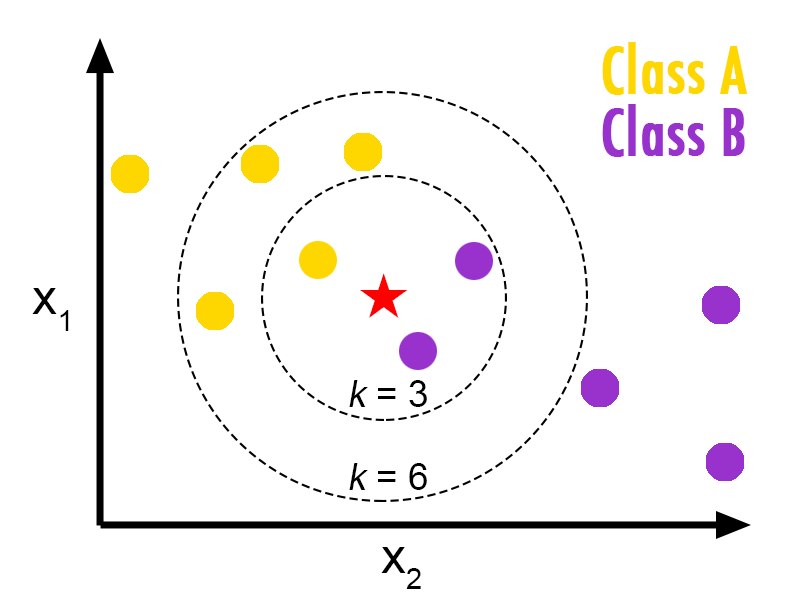
\includegraphics[height=0.8\textheight]{figures/knn} \\
        {\scriptsize%
         From Burton DeWilde's blog}
        \end{center}}
\end{frame}

\begin{frame}{Choice of $k$}
    \begin{itemize}
        \item Larger $k$ $\rightarrow$ smoother boundaries, less `noisy'
        \item If $k = N$, we always predict the majority class
    \end{itemize}
    \vfill
    \begin{center}
        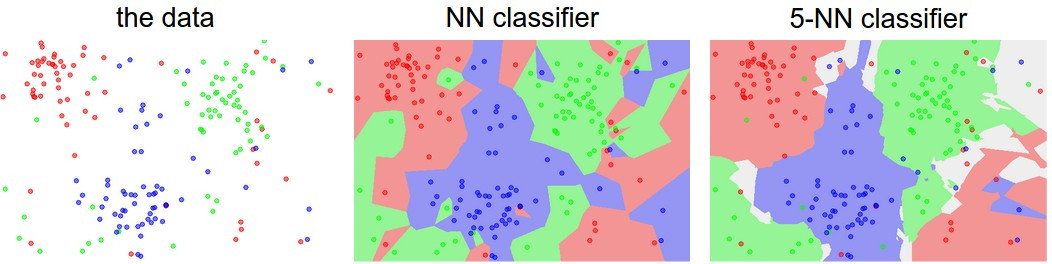
\includegraphics[width=\textwidth]{figures/k_effect} \\
        {\scriptsize%
         From \textit{CS231n: Convolutional Neural Networks for Visual Recognition}}
    \end{center}
\end{frame}

\begin{frame}{Minkowski distance}
    \[
        \left( \sum_{i} \left| x_{i} - y_{i} \right|^{p} \right)^{\!1/p}
    \]
    \vfill
    \begin{center}
        \renewcommand*{\arraystretch}{1.5}
        \begin{tabular}{lll}
            \toprule
            $p = 1$ & Manhattan distance & $\sum_{i} \left| x_{i} - y_{i} \right|$ \\
            $p = 2$ & Euclidean distance & $\sqrt{\sum_{i} \left( x_{i} - y_{i} \right)^{2}}$ \\
            \bottomrule
        \end{tabular}
    \end{center}
\end{frame}

\begin{frame}{Weight of neighbours}
    \begin{block}{Uniform weights}
        \begin{itemize}
            \item All $k$ neighbours contribute equally to the prediction
            \item Actual distance to each is ignored
        \end{itemize}
    \end{block}
    \vfill
    \begin{block}{Distance weights}
        \begin{itemize}
            \item Contributions are weighted by $1 / \text{distance}$
            \item Closer neighbours influence the prediction more
        \end{itemize}
    \end{block}
\end{frame}

\begin{frame}{Curse of dimensionality}
    As the number of variables (coordinates) increases\ldots
    \begin{itemize}
        \item The volume of the space increases
        \item Pairwise distances become more similar $\rightarrow$ sparsity
        \item Some samples have huge neighbourhoods $\rightarrow$ `hubs'
    \end{itemize}
\end{frame}

\section{Metrics}

\begin{frame}{Classification accuracy}
    \begin{block}{Classification accuracy}
        \begin{itemize}
            \item Percentage of \alert{correct} predictions
            \item Higher is better
        \end{itemize}
    \end{block}
    \vfill
    \begin{block}{Classification error}
        \begin{itemize}
            \item Percentage of \alert{incorrect} predictions
                  (inverse of accuracy)
            \item Lower is better
        \end{itemize}
    \end{block}
\end{frame}

\newsavebox{\TP}
\savebox{\TP}{%
    \begin{minipage}[c]{2cm}
        \centering
        \vspace{0.25cm}
        {\Large\color{mDarkTeal}\cmark} \\[-0.25cm]
        {\tiny%
         True positive}
        \vspace{0.25cm}
    \end{minipage}}

\newsavebox{\TN}
\savebox{\TN}{%
    \begin{minipage}[c]{2cm}
        \centering
        \vspace{0.25cm}
        {\Large\color{mDarkTeal}\cmark} \\[-0.25cm]
        {\tiny%
         True negative}
        \vspace{0.25cm}
    \end{minipage}}

\newsavebox{\FP}
\savebox{\FP}{%
    \begin{minipage}[c]{2cm}
        \centering
        \vspace{0.25cm}
        {\Large\color{mDarkBrown}\xmark} \\[-0.25cm]
        {\tiny%
         False positive}
        \vspace{0.25cm}
    \end{minipage}}

\newsavebox{\FN}
\savebox{\FN}{%
    \begin{minipage}[c]{2cm}
        \centering
        \vspace{0.25cm}
        {\Large\color{mDarkBrown}\xmark} \\[-0.25cm]
        {\tiny%
         False negative}
        \vspace{0.25cm}
    \end{minipage}}

\begin{frame}[fragile]{Confusion matrix}
    \begin{center}
        \begin{tabular}{cc|cc}
                &     & \multicolumn{2}{c}{\textbf{Predicted}} \\
                &     & $1$          & $0$ \\ \hline
            \multirow{2}{*}[-0.75em]{\rotatebox[origin=c]{90}{\textbf{Actual}}}%
                & $1$ & \usebox{\TP} & \usebox{\FN} \\
                & $0$ & \usebox{\FP} & \usebox{\TN} \\
        \end{tabular}
    \end{center}
    \vfill
    \begin{itemize}
        \item Gives a better understanding of behaviour
        \item Can be used to define multiple performance metrics
    \end{itemize}
\end{frame}

\begin{frame}{Sensitivity and specificity}
    \vspace{-1em}
    \begin{columns}[T]
        \begin{column}{0.5\textwidth}
            \begin{center}
                \textbf{Sensitivity} \\[-0.25em]
                {\small%
                 (a.k.a.\ true positive rate)}
                \[
                    \frac{\sum\,\text{True positive}}{\sum\,\text{Actual} = 1}
                \]
            \end{center}
            \vfill
            \onslide<2->{%
                \begin{block}{Perfect sensitivity}
                    \begin{itemize}
                        \item All sick identified as sick
                        \item Negative test result definitely rules out disease
                    \end{itemize}
                \end{block}}
        \end{column}
        \begin{column}{0.5\textwidth}
            \begin{center}
                \textbf{Specificity} \\[-0.25em]
                {\small%
                 (a.k.a.\ true negative rate)}
                \[
                    \frac{\sum\,\text{True negative}}{\sum\,\text{Actual} = 0}
                \]
            \end{center}
            \vfill
            \onslide<3->{%
                \begin{block}{Perfect specificity}
                    \begin{itemize}
                        \item No healthy identified as sick
                        \item Positive test result useful for ruling in disease
                    \end{itemize}
                \end{block}}
        \end{column}
    \end{columns}
    \vfill
    \onslide<4->{%
        \begin{center}
            \alert{Can we maximise both at the same time?}
        \end{center}}
\end{frame}

\begin{frame}{`Perfect' border control}
    \begin{block}{100\% sensitivity}
        \begin{itemize}
            \item `Everyone is a terrorist!'
            \pause
            \item All terrorists are stopped $\rightarrow$ 100\% sensitivity
            \pause
            \item No one can enter the country! $\rightarrow$ 0\% specificity
        \end{itemize}
    \end{block}
    \vfill\pause
    \begin{block}{100\% specificity}
        \begin{itemize}
            \item `No one is a terrorist!'
            \pause
            \item All non\hyp{}terrorists are allowed in $\rightarrow$ 100\% specificity
            \pause
            \item All terrorists are also allowed into the country! $\rightarrow$ 0\% sensitivity
        \end{itemize}
    \end{block}
\end{frame}

\begin{frame}{ROC and AUC}
    \vspace{-1em}
    \begin{columns}[T]
        \begin{column}{0.5\textwidth}
            \begin{center}
                \textbf{Receiver Operating Characteristic (ROC) curve} \\
                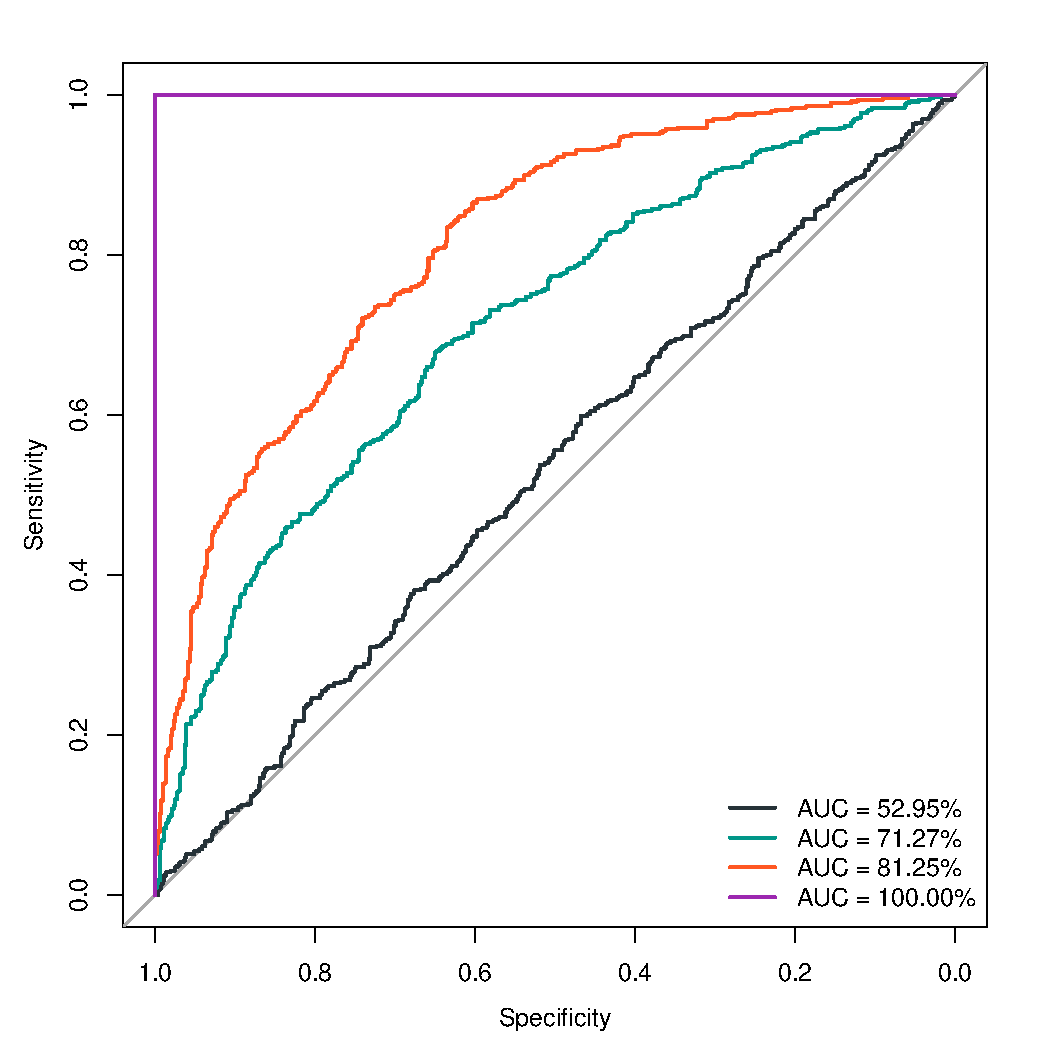
\includegraphics[height=0.6\textheight]{figures/roc} \\
                Sensitivity \textit{vs} ($1 - \text{specificity}$) \\
                $\rightarrow$ TP rate \textit{vs} FP rate
            \end{center}
        \end{column}
        \pause
        \begin{column}{0.5\textwidth}
            \begin{center}
                \vspace{1ex}
                \textbf{Area Under the Curve (AUC)} \\[\medskipamount]
            \end{center}
            \begin{itemize}
                \item Probability that
                      $\text{Prediction}\!\left( \text{actual 1} \right) > \text{Prediction}\!\left( \text{actual 0} \right)$
                \item Random guess \\
                      $\rightarrow$ AUC = 50\% (diagonal)
                \item Higher is better
            \end{itemize}
        \end{column}
    \end{columns}
\end{frame}

\section{Cost\hyp{}benefit analysis}

\begin{frame}{Cost\hyp{}benefit analysis}
    \begin{itemize}
        \item Assume that the four possible outcomes of a classification problem
              have (numerical) \alert{benefits and costs}
              \begin{description}
                  \item[$> 0$] desirable (e.g.\ profit)
                  \item[$= 0$] neutral
                  \item[$< 0$] undesirable (e.g.\ loss) \\[\bigskipamount]
              \end{description}
        \item These `benefits and costs' needn't be symmetrical
    \end{itemize}
\end{frame}

\newsavebox{\TPexA}
\savebox{\TPexA}{%
    \begin{minipage}[c]{2cm}
        \centering
        \vspace{0.5cm}
        20\%
        \vspace{0.5cm}
    \end{minipage}}

\newsavebox{\TNexA}
\savebox{\TNexA}{%
    \begin{minipage}[c]{2cm}
        \centering
        \vspace{0.5cm}
        50\%
        \vspace{0.5cm}
    \end{minipage}}

\newsavebox{\FPexA}
\savebox{\FPexA}{%
    \begin{minipage}[c]{2cm}
        \centering
        \vspace{0.5cm}
        10\%
        \vspace{0.5cm}
    \end{minipage}}

\newsavebox{\FNexA}
\savebox{\FNexA}{%
    \begin{minipage}[c]{2cm}
        \centering
        \vspace{0.5cm}
        20\%
        \vspace{0.5cm}
    \end{minipage}}

\newsavebox{\TPexB}
\savebox{\TPexB}{%
    \begin{minipage}[c]{2cm}
        \centering
        \vspace{0.5cm}
        30\%
        \vspace{0.5cm}
    \end{minipage}}

\newsavebox{\TNexB}
\savebox{\TNexB}{%
    \begin{minipage}[c]{2cm}
        \centering
        \vspace{0.5cm}
        55\%
        \vspace{0.5cm}
    \end{minipage}}

\newsavebox{\FPexB}
\savebox{\FPexB}{%
    \begin{minipage}[c]{2cm}
        \centering
        \vspace{0.5cm}
        10\%
        \vspace{0.5cm}
    \end{minipage}}

\newsavebox{\FNexB}
\savebox{\FNexB}{%
    \begin{minipage}[c]{2cm}
        \centering
        \vspace{0.5cm}
        5\%
        \vspace{0.5cm}
    \end{minipage}}

\begin{frame}{Planning an outdoor activity}
    \only<1>{%
        You have 20 people enrolled in an outdoor activity paying £30 each
        \begin{itemize}
            \item Before the activity, you check the weather forecast and either:
                  \begin{itemize}
                      \item Go ahead, which costs you £5 per participant
                      \item Cancel and refund the participants in full
                  \end{itemize}
            \item If you decide to go ahead, the day of the activity it will
                  either:
                  \begin{itemize}
                      \item Be sunny, in which case you get to keep the profit
                      \item Rain, in which case you'll have to refund the
                            participants in full
                  \end{itemize}
        \end{itemize}
        What is the `benefits and costs' matrix?}
    \only<2>{%
        \begin{columns}[t]
            \begin{column}{0.5\textwidth}
                \begin{center}
                    \textbf{Free weather forecast} \\[\bigskipamount]
                    \begin{tabular}{cc|cc}
                            &       & \multicolumn{2}{c}{\textbf{Forecast}} \\
                            &       & \Sun           & \Rain \\ \hline
                        \multirow{2}{*}[-0.75em]{\rotatebox[origin=c]{90}{\textbf{Actual}}}%
                            & \Sun  & \usebox{\TPexA} & \usebox{\FNexA} \\
                            & \Rain & \usebox{\FPexA} & \usebox{\TNexA} \\
                    \end{tabular}
                \end{center}
            \end{column}
            \begin{column}{0.5\textwidth}
                \begin{center}
                    \textbf{Weather forecast costing £15} \\[\bigskipamount]
                    \begin{tabular}{cc|cc}
                            &       & \multicolumn{2}{c}{\textbf{Forecast}} \\
                            &       & \Sun           & \Rain \\ \hline
                        \multirow{2}{*}[-0.75em]{\rotatebox[origin=c]{90}{\textbf{Actual}}}%
                            & \Sun  & \usebox{\TPexB} & \usebox{\FNexB} \\
                            & \Rain & \usebox{\FPexB} & \usebox{\TNexB} \\
                    \end{tabular}
                \end{center}
            \end{column}
        \end{columns}
        \begin{itemize}
            \item What are the sensitivity and specificity?
            \item What is the expected profit?
        \end{itemize}}
\end{frame}

\end{document}

